\chapter{Método tradicional}

O sistema de segurança na fábrica consiste na detecção de pessoas sob a área da ponte. Esse é um problema de localização de objetos, mais especificamente, de detecção de pessoas. Tradicionalmente divide-se essa tarefa em três técnicas de visão computacional: obtenção de candidatos a objeto, obter descrição de cada candidato e então validar a amostra através de classificador. Essa solução foi baseada no trabalho de \cite{rauter}.

Para essa aplicação, recomenda-se a utilização de imagens de profundidade, em que o valor dos pixels indicam a distância entre a câmera e o objeto em questão. Isso se deve ao fato de esse sensor fornecer uma medida independente de luminosidade e variações de cor ou textura, se comparada à uma câmera RGB tradicional. Três câmeras foram compradas e avaliadas: \textit{ASUS XtionPRO}, \textit{Orbbec Astra PRO} e \textit{Stereolabs ZED}. As duas primeiras funcionam com o princípio de laser estruturado, já a última funciona baseado em visão estéreo (duas câmeras). Através de testes determinou-se que as maiores distâncias detectadas foram de 4m, 5m e 20m respectivamente. Dado que a câmera será instalada a 6m do chão, em visão superior, optou-se por utilizar a câmera \textit{ZED}.

As imagens recebidas da câmera precisam ser préprocessadas de forma a obter um mapa de distâncias, que é a imagem de profundidade. Isso é feito pela biblioteca fornecida pela \textit{Stereolabs}. Em seguida, inverte-se a imagem (subtrai-se cada pixel da distância da câmera) de maneira que cada pixel forneça a altura em relação ao chão do objeto por ele representado. Além disso remove-se pixels cujas distâncias não foram corretamente estimadas e o resultado é uma imagem cujos valores representam a altura dos objetos em milimetros.

\section{Obtenção de candidatos}
O primeiro passo consiste em obter candidatos a pessoas, como a vista é superior, candidatos a cabeças. Em uma aplicação tradicional, com câmeras RGB esse processo dividiria a imagem em pequenos blocos de tamanhos que se espera para uma cabeça, sem qualquer informação sobre o posicionamento, isto é, varrendo uma "janela imaginária`` pela imagem.

Para aprimorar esse método, assume-se a hipótese de que cabeças serão os objetos mais altos de uma vizinhança, se destacando na cena dos demais objetos. Embora ela não seja sempre verdadeira, ao se verificar que existem máquinas altas, é um método mais eficiente de selecionar candidatos pois utiliza informação prévia da cena.

Aplica-se o método de máximos locais: a imagem é dividida em quadrados de áreas iguais. Para cada quadrado percorre-se os pixels e seleciona-se o maior deles, se este pixel for único no conjunto ele é considerado um ponto candidato à cabeça. Esse processo resulta num conjunto de pontos que determinam candidados à cabeças.

O tamanho dos quadrados que dividem a imagem é fundamental nessa etapa: se forem muito grandes há alta probabilidade de se perder cabeças visto que na cena existem máquinas altas. Por outro lado, se forem muito pequenos, existirão muitos candidatos e o processo se torna lento. Esse tamanho é calculado utilizando a distância focal da câmera, a altura média de pessoas e o tamanho padrão de cabeças através da equação \ref{eq:cam-proj}.

\begin{equation}
	\label{eq:cam-proj}
	s_w = \frac{f}{d} \cdot s_r
\end{equation}

Em seguida, é necessário determinar um quadrado que delimite a cabeça de forma centralizada. Para obter o tamanho do quadrado, novamente utiliza-se a equação \ref{eq:cam-proj}, porém dessa vez utilizando o valor do pixel encontrado para aquele candidato como altura. Tem-se então um quadrado de tamanho apropriado com o pixel máximo no centro, porém em poucos casos esse quadrado centraliza a cabeça.

Utiliza-se um processo de centralização baseado em \textit{mean shift}, que permite iterativamente localizar o máximo de uma função probabilidade dado uma máscara. Nesse caso, uma interpretação do procedimento é mover o quadrado mantendo suas dimensões fixas para o centróide dos pixels que estão em seu interior. Intuitivamente, percebe-se que os pixels de valor mais elevado terão maior peso, portanto, espera-se que o quadrado seja centralizado sob parte central da cabeça.

Atualiza-se o centro do retângulo, $p \gets m(p)$, como explicitado na equação \ref{eq:mean-shift}, onde $I$ é a imagem e $S(p)$ é o conjunto dos pixels no quadrado de centro $p$.
\begin{equation}
	\label{eq:mean-shift}
	m(p) = \frac{\sum_{p_i \in S(p)} I(p_i)p_i}{\sum_{p_i \in S(p)} I(p_i)}
\end{equation}

\begin{figure}[h]
\caption{Pontos em azul são máximos locais e os quadrados vermelhos indicam os candidatos centralizados}
\centering
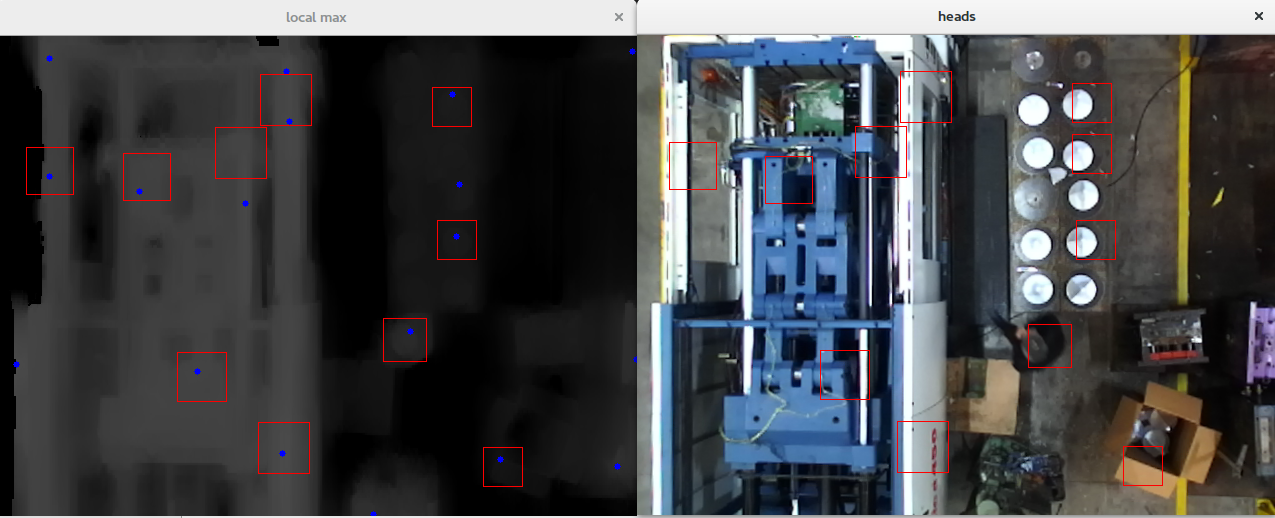
\includegraphics[width=0.8\textwidth]{tradicional/candidatos}
\label{fig:candidatos}
\end{figure}

Ao final dessa etapa, conta-se com uma lista de candidatos representados pelo \textit{patch} da imagem correspondente, como ilustrado na figura \ref{fig:candidatos} pelos quadrados em vermelho.

\section{Descritores}
No trabalho de referência se destacam dois descritores: grades simples e grades circulares. Observa-se que para todos os descritores a característica importante de representação está nos desníveis da cabeça em relação ao resto do corpo, que se dá de maneira praticamente circular. Portanto, objetiva-se encontrar uma maneira de evidenciar quando e em que grau esse tipo de padrão acontece.

O primeiro divide o candidato em blocos, com uma quantidade ímpar em cada dimensão, como ilustrado na figura \ref{fig:descritores}. Então calcula-se a média dos pixels em cada um dos blocos. Em seguida subtrai-se de todos os blocos a média do bloco central e por fim gera-se um histograma dos valores resultantes, que corresponde à descrição do candidato. Para esse descritor em específico, fixou-se a quantidade de blocos em 7 para cada dimensão, 49 blocos no total pois avaliou-se que para o tamanho dos candidatos foi a representação mais adequada.

Já o segundo método proposto na referência propõe que uma série de blocos seja disposta circularmente sobre a imagem candidata e que o mesmo procedimento do primeiro extrator seja realizado. O objetivo seria dar ao descritor uma maior invariância à rotação, dada a distribuição dos blocos. Porém esse extrator é difícil de generalizar devido à variação do tamanho dos candidatos.

Outro modelo é criado: descritor de anéis concêntricos. A ideia é similar, porém ao invés de se dispor blocos de maneira circular, utilizam-se coroas que partem desde o centro da imagem até as extremidades. Calcula-se a média dos pixels que ocupam cada coroa e por fim diferencia-se o vetor das médias, obtendo então a descrição para o candidato. É possível observar o padrão dos anéis na figura \ref{fig:descritores}, cada cor representa um grupo de pixels cuja média é calculada. Para esse descritor utilizou-se um diferente número de anéis para avaliar o nível de descrição.

\begin{figure}[h]
\caption{Ilustração dos descritores: grades simples e anéis concêntricos.}
\centering
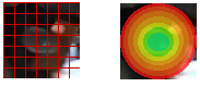
\includegraphics[width=0.8\textwidth]{tradicional/descritores}
\label{fig:descritores}
\end{figure}

\section{Classificação}
